\addtocontents{toc}{\protect\vspace{10pt}}
\section{Chapter 4: Correlation and regression}

\learningobjectives{
    \item Calculating covariance and correlation by hand
    \item Testing hypotheses about a correlation by hand
    \item Calculating and testing a correlation in R
    \item Testing hypotheses using linear regression in R
    \item Making predictions using linear regression in R
}

% To add an assignment to the chapter, create a file in the folder "Assignments" and insert the link below

%%%%%%%%%%%%%%%%%%%%%%%%%%%%%%%%%%%%%%%%%%%%%%%%%%%%%%%%%%%%%%%%%%%%%%%%%%%
% Assignment 4.1: Calculating covariance and correlation by hand
%%%%%%%%%%%%%%%%%%%%%%%%%%%%%%%%%%%%%%%%%%%%%%%%%%%%%%%%%%%%%%%%%%%%%%%%%%%

\handassignment{Assignment 4.1: Calculating covariance and correlation by hand}

The manager of a local branch of a supermarket chain in the Netherlands has had a bad year last year and wants to improve their sales. Her co-worker has brought up the idea to spend more money on advertising in the neighborhoods that are further away from the store. The co-worker thinks that customers that live further away might visit the supermarket less frequently. He believes that making an effort to attract these people may prove to be profitable for the store. Realizing that her branch currently does not spend a notable amount of money on advertising at all, the manager is interested to know about the \concept{relationship} between the distance a customer lives from the store and the average number of times they visit the store per week. \\

The manager requests her co-worker to ask the customers at his counter some questions when they check out at his counter. He is instructed to ask them a) how many times, on average, they visit the store per week and b) the number of kilometers they live from the store. The co-worker asks eight customers and reports the findings to his manager. \\

\question{
    4.1 a
}{
    What kind of \concept{relationship} do you expect to see? Formulate your answer in terms of the direction of the \concept{relationship}.
}

\twolineanswerbox{4.1a}

The manager sits down with her co-worker, writes down the numbers, and creates a scatter plot of the data. She displays the distance a customer lives from the store (in kilometers) on the \textit{x-axis} and their average number of visits per week on the \textit{y-axis}. 

\clearpage % Page break

\begin{minipage}[t]{0.4\textwidth}
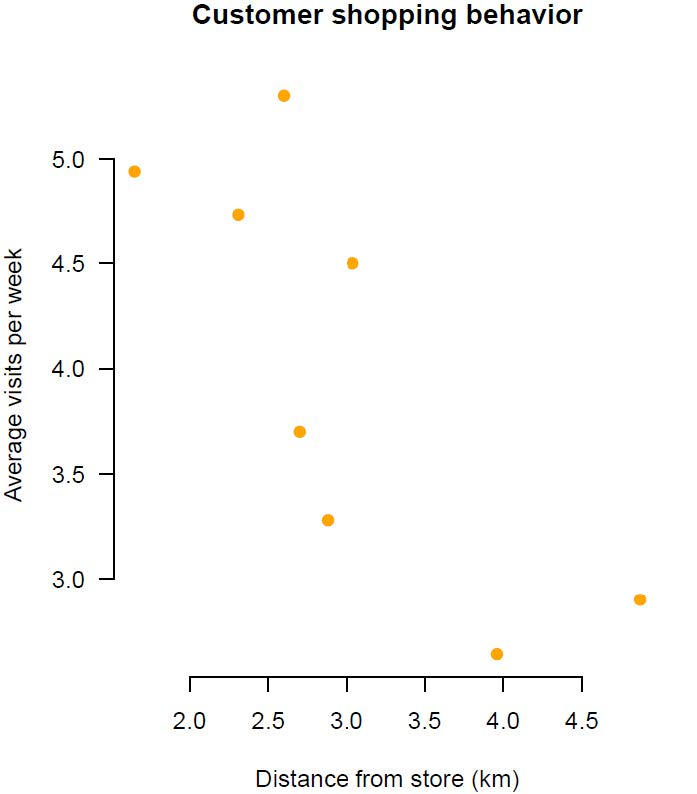
\includegraphics[width=\textwidth]{Files/Images/covariance.jpg}
\end{minipage}%
\begin{minipage}[t]{0.6\textwidth}
\vspace*{-7cm}
\begin{center}
    \begin{tabular}{|c|c|c|c|c|c|}
    \hline 
    $i$ & $x_i$ & $y_i$ & $(x_i - \bar{x})$ & $(y_i - \bar{y})$ & $(x_i - \bar{x})(y_i - \bar{y})$ \tstrut\bstrut\\
    \hline
    1 & 4.87 & 2.90 & & &  \tstrut\bstrut\\
    \hline
    2 & 3.04 & 4.50 & & &  \tstrut\bstrut\\
    \hline
    3 & 1.65 & 4.94 & & &  \tstrut\bstrut\\
    \hline
    4 & 2.88 & 3.28 & & &  \tstrut\bstrut\\
    \hline
    5 & 2.31 & 4.73 & & &  \tstrut\bstrut\\
    \hline
    6 & 3.96 & 2.64 & & &  \tstrut\bstrut\\
    \hline
    7 & 2.70 & 3.70 & & &  \tstrut\bstrut\\
    \hline
    8 & 2.60 & 5.30 & & &  \tstrut\bstrut\\
    \hline
    \end{tabular}
    \end{center}
    
    \hspace*{.5cm} $\bar{x} = $  ............. \hspace*{1cm} $\sum (x_i - \bar{x})(y_i - \bar{y}) = $  ............. \\
    \\
    \hspace*{.5cm} $\bar{y} = $ ............. \hspace*{3.1cm} $n - 1 = $  ............. \\
    \\
    \hspace*{6.5cm} $s_{xy} = $  ............ \\
\end{minipage}%

\question{
    4.1 b
}{
    Use the table above to calculate and fill in the \concept{covariance} $s_{xy}$ between the customer’s distance from the store and their average number of visits per week. 
}

\hint{Hint 4.1: you can find the complete formula for the \concept{covariance} in the formula sheet.}

\question{
    4.1 c
}{
    Interpret the \concept{covariance} from these data. What can you say about the \concept{relationship} between the distance from the store and the average number of visits per week on the basis of this measure?
}

\threelineanswerbox{4.1c}

The \concept{covariance} $s_{xy}$ is a useful measure to get an idea about the extent to which two \concept{variables} change together, but it also has some disadvantages when using it as a measure of the strength of a \concept{relationship}. 

\clearpage % Page break

\question{
    4.4 d
}{
    Explain the disadvantage of using the \concept{covariance} $s_{xy}$ as a measure for the strength of this \concept{relationship}. Consider in your answer what would have happened if the co-worker asked the customers how many meters they lived from the store.
}

\threelineanswerbox{4.1d}

To reliably measure the strength of the \concept{relationship}, the manager wants to \concept{standardize} the \concept{covariance} $s_{xy}$ to find out the \concept{correlation} coefficient $r_{xy}$. To do this, she first needs to calculate the sample \concept{standard deviation} of the distance from the store in kilometers ($s_x$) and the sample \concept{standard deviation} of the average number of visits per week($s_y$). \\

\question{
    4.1 e
}{
    Calculate $s_x$ and $s_y$ for the data that the co-worker collected. 
}

\hint{Hint 4.2: you can find the formula for the \concept{standard deviation} in the formula sheet.}

\emptyanswerbox{
    4.1e
}{
    $s_x$: \shortanswerline \hspace*{3cm} $s_y$: \shortanswerline
}

\question{
    4.1 f
}{
    Use the sample \concept{standard deviations} and the sample \concept{covariance} to calculate the sample \concept{correlation} $r_{xy}$.
}

\hint{Hint 4.3: you can find the formula for the \concept{correlation coefficient} $r_{xy}$ in the formula sheet.}

\emptyanswerbox{
    4.1f
}{
    $r_{xy}$: \shortanswerline
}

\question{
    4.1 g
}{
   Interpret the \concept{correlation coefficient}. Is this a strong \concept{relationship}?
}

\onelineanswerbox{4.1g}

\clearpage % Page break
%%%%%%%%%%%%%%%%%%%%%%%%%%%%%%%%%%%%%%%%%%%%%%%%%%%%%%%%%%%%%%%%%%%%%%%%%%%
% Assignment 4.2: Testing hypotheses about a correlation by hand
%%%%%%%%%%%%%%%%%%%%%%%%%%%%%%%%%%%%%%%%%%%%%%%%%%%%%%%%%%%%%%%%%%%%%%%%%%%

\handassignment{Assignment 4.2: Testing hypotheses about a correlation by hand}

The store manager looks at the results of her calculations and sees some potential for increasing the sales of her branch. However, before she starts spending more money on advertising in these to hard-to-reach neighborhoods, she wants to gain reasonable assurance that her results can be generalized to all of her potential customers. Therefore, she wants to test the hypothesis that, with 95\% confidence, this \concept{correlation} is truly negative in the entire \concept{population} of customers. \\

\question{
    4.2 a
}{
    Formulate the \concept{null hypothesis} $H_0$ and \concept{alternative hypothesis} $H_1$ for the manager’s test of the \concept{population correlation coefficient} $\rho_{xy}$.  
}

\hint{Hint 4.4: Think about whether this is a one-sided test or a two-sided test?}

\hypothesesbox{4.2a}

\question{
    4.2 b
}{
    Write down the relevant information that appeared in assignment 4.1. Use the symbols $N$, $n$, $r_{xy}$, $\rho_{xy}$
}

\hint{Hint 4.5: Not all symbols are known.}

\emptyanswerbox{
    4.2b
}{
        $N$: \shortanswerline \hspace{1cm} \quad $r_{xy}$: \shortanswerline
            \answerbreak
            \hspace*{1pt}$n$: \shortanswerline \hspace{1cm} \quad $\rho_{xy}$: \shortanswerline
}

\question{
    4.2 c
}{
    Find out the \concept{critical z-value} that is required to reject $H_0$ with 95\% confidence.
}

\emptyanswerbox{
    4.2c
}{
    $z_{critical}$: \shortanswerline
}

\question{
    4.2 d
}{
    Calculate the sample \concept{z-value} for the \concept{correlation coefficient} $r_{xy}$.
}

\hint{Hint 4.6: You can find the formula for the \concept{z-value} of a \concept{correlation} in the formula sheet.}

\clearpage % Page break

\emptyanswerbox{
    4.2d
}{
    $z_{xy}$: \shortanswerline
}

\question{
    4.2 e
}{
    Draw the conclusion for the manager. Include the following four elements:
    \begin{itemize}
    \item[$\square$] Show how the calculated \concept{z-value} relates to the \concept{critical z-value}.
    \item[$\square$] Discuss whether $H_0$ is rejected or not.
    \item[$\square$] Describe what this tells us about $\rho_{xy}$.  
    \item[$\square$] Describe what type of error is relevant \textit{(type-I or type-II)}.
\end{itemize}
}

\sixlineanswerbox{4.2e}

\clearpage % Page break
%%%%%%%%%%%%%%%%%%%%%%%%%%%%%%%%%%%%%%%%%%%%%%%%%%%%%%%%%%%%%%%%%%%%%%%%%%%
% Assignment 4.2: Testing hypotheses about a correlation by hand
%%%%%%%%%%%%%%%%%%%%%%%%%%%%%%%%%%%%%%%%%%%%%%%%%%%%%%%%%%%%%%%%%%%%%%%%%%%

\rassignment{Assignment 4.3: Calculating and testing a correlation in R}

The supermarket manager believes she has found a weakness in the distribution policy of the supermarket and believes that more stores should be built nationwide to be more active in other areas. To strengthen her case for the board of directors, she has asked permission to execute her survey in 100 stores in the Netherlands to gather data of 1000 customers. She wants to confirm her \concept{hypothesis} that in the entire Netherlands, there is a negative \concept{relationship} between the distance a customer lives from their supermarket, and the number of times they visit their supermarket. \\

For this assignment, you need the data file \dataset{localSupermarket.csv}, which contains a population of 1,000 observations. \\

\question{
    4.3 a
}{
    Use the \rcode{read.csv()} function (and \rcode{setwd()} function if you prefer) to import the data set into a data frame called \code{dataset6}.
}

\rcodeanswertiny{4.3a}

\question{
    4.3 b
}{
    Use the \rcode{cov()} and \rcode{cor()} functions to calculate the \concept{covariance} $s_{xy}$ and the \concept{correlation} $r_{xy}$ of the columns \rcode{Distance} and \rcode{AvgVisits}.
}

\rcodeanswersmall{4.3b}
\emptyanswerbox{
    4.3 b
}{
    Covariance: \shortanswerline
    \answerskip
    Correlation: \shortanswerline
}

\question{
    4.3 c
}{
    Use the function \rcode{cor.test()} to test for a negative \concept{relationship} in this \concept{population}. Use \rcode{?cor.test} to get help about the function arguments. Can you confirm the value of the \concept{correlation} that you found in assignment 4.3b?
}

\rcodeanswersmall{4.3c}

\clearpage % Page break

Instead of using the \concept{standard normal distribution} $N(\mu = 0, \sigma = 1)$ and a \concept{z-value} for testing $\rho_{xy}$ against any value, you can simplify the procedure when you are testing a \concept{correlation coefficient} testing against the value zero (which is almost always the case). In such a case, you can use the \concept{t-distribution} for calculating a \concept{t-value} for the significance of $\rho_{xy}$ against a value of zero. The \concept{t-distribution} is almost identical to the \concept{normal distribution}. However, where the \concept{normal distribution} is defined by its \concept{mean} ($\mu$) and its \concept{standard deviation} ($\sigma$), the \concept{t-distribution} is defined by its degrees of freedom ($df_{n - 1}$). \\

\begin{center}
    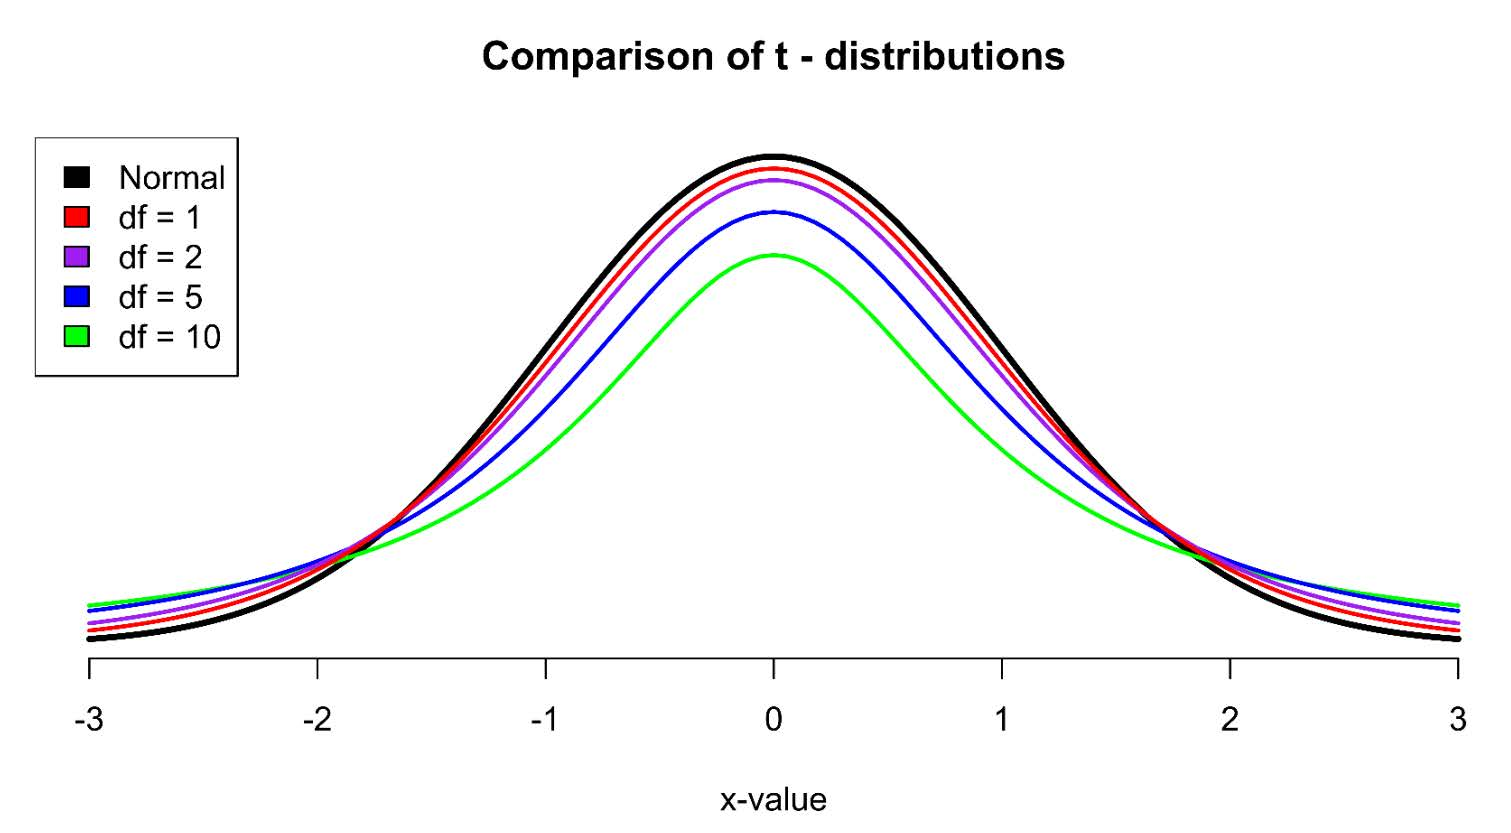
\includegraphics[width=.9\textwidth]{Files/Images/tdistributions.jpg}
\end{center}

Use the following \texttt{R} code to create a figure of the \concept{t-distribution} with $df = 3$. \\

\codeblock{curve(dnorm(x, mean = 0, sd = 1), from = -3, to = 3, ylab = \textquotesingle Density\textquotesingle)\\
curve(dt(x, df = 3), from = -3, to = 3, add = TRUE, col = \textquotesingle red\textquotesingle)
}

\question{
    4.3 d
}{
    Which line represents the \concept{normal distribution} in the figure that was drawn? And which line represents the \concept{t-distribution}? Can you explain what the difference between the two distributions is in terms of their shape? What happens when you increase the \concept{degrees of freedom} (\rcode{df}) in the \rcode{dt()} function?
}

\twolineanswerbox{4.3d}

\question{
    4.3 e
}{
    Calculate the \concept{degrees of freedom} and the \concept{t-value} for the \concept{correlation coefficient} between \rcode{Distance} and \rocde{AvgVisits}.
}

\hint{Hint 4.7: You can find the formula for the \concept{degrees of freedom} and the \concept{t-value} of a \concept{correlation} in the formula sheet.}

\clearpage % Page break

\rcodeanswertiny{4.3e}

\emptyanswerbox{
    4.3e
}{
    $df$: \shortanswerline \hspace*{3cm} $t_{xy}$: \shortanswerline
}

\question{
    4.3 f
}{
    Where do you find the \concept{t-value} that you calculated in assignment 4.3e in the output of the \rcode{cor.test()} function from assignment 4.3c?
}

\onelineanswerbox{4.3f}

\question{
    4.3 g
}{
    What is the \concept{p-value} for this hypothesis test? Interpret this \concept{p-value} with respect to the confidence used and give a conclusion on the hypotheses. Include the following elements:
    \begin{itemize}
        \item[$\square$] Discuss what the \concept{p-value} is for this test.
    \item[$\square$] Discuss whether $H_0$ is rejected or not.
    \item[$\square$] Describe what this tells us about $\rho_{xy}$.  
    \item[$\square$] Describe what type of error is relevant \textit{(type-I or type-II)}.
\end{itemize}
}

\sixlineanswerbox{4.3g}

\clearpage % Page break
%%%%%%%%%%%%%%%%%%%%%%%%%%%%%%%%%%%%%%%%%%%%%%%%%%%%%%%%%%%%%%%%%%%%%%%%%%%
% Assignment 4.4: Testing hypotheses using linear regression in R
%%%%%%%%%%%%%%%%%%%%%%%%%%%%%%%%%%%%%%%%%%%%%%%%%%%%%%%%%%%%%%%%%%%%%%%%%%%

\rassignment{Assignment 4.4: Testing hypotheses using linear regression in R}

A manager from a local supermarket wants to increase the sustainability of her store. Since the supermarket is located in a farm village that has easy access to milk, many milk cartons are not sold, expire, and have to be thrown away. From common sense, the manager suspects that decreasing the price of milk will result in more sales, and thus fewer milk cartons that get thrown away. In order to increase her sustainability through this method, the manager sets out to find out if a decrease in the price per carton of milk will result in fewer milk cartons thrown away on an average day. She also wants to predict her decrease in waste when she lowers the price of a milk carton by 30 cents. \\

The manager goes to the company headquarters and asks the prices of milk (they vary) in every branch of the supermarket chain in the Netherlands. She also asks the average number of milk cartons thrown away per day of each branch. \\

For this assignment, you need the data file \dataset{nationalSupermarket.csv}, which contains the full \concept{population} of 200 stores of the supermarket chain in the Netherlands. \\

\question{
    4.4 a
}{
    Use the \rcode{read.csv()} function (and \rcode{setwd()} function if you prefer) to import the data set into a data frame called \rcode{dataset7}.
}

\rcodeanswertiny{4.4a}

\question{
    4.4 b
}{
    Create a scatter plot of the data. Put the price per milk carton (\rcode{Price}) on the \textit{x-axis} and the average number of milk cartons that was thrown away (\rcode{AvgWasted}) on the \textit{y-axis}.
}

\rcodeanswersmall{4.4b}

The \rcode{lm()} function is used to fit a linear model (linear regression) in \texttt{R}. It requires that you specify a \rcode{formula} that tells the function what the \concept{regression equation} is. If you want to fit a \concept{model} where you predict an outcome variable \rcode{Y} on the basis of one predictor variable \rcode{X}, the formula is as follows: \\

\begin{center}
    \textbf{Formula on paper: }$Y = \beta_0 + \beta_1 \times X$ 
    \hspace*{2cm}
    \textbf{Formula in R: }\rcode{Y {\raise.17ex\hbox{$\scriptstyle\sim$}} 1 + X}
\end{center}

\question{
    4.4 c
}{
    Write down the \concept{regression equation} for a linear model where you predict the average number of thrown away milk cartons per day (\rcode{AvgWasted}) on the basis of the price per milk carton (\rcode{Price}). 
}

\emptyanswerbox{
    4.4c
}{
    AvgWasted = \longanswerline
}

\clearpage % Page break

A linear \concept{model} with these variables can be fitted in \texttt{R} by calling the \rcode{lm()} function with the \rcode{formula} and the \rcode{dataset} (see the \texttt{R} code below). The variables \rcode{X} and \rcode{Y} should correspond to the names of the corresponding variables in your \rcode{dataset}. \\

\codeblock{lm(formula = Y {\raise.17ex\hbox{$\scriptstyle\sim$}} 1 + X, data = dataset)}

\question{
    4.4 d
}{
    Fit a linear \concept{model} where you use the data in \rcode{dataset7} to predict the average number of thrown away milk cartons per day (\rcode{AvgWasted}) on the basis of the price per milk carton (\rcode{Price}). Store this \concept{model} in an object called \rcode{lmfit}.
}

\rcodeanswertiny{4.4d}

Now run the following code in \texttt{R}: \\

\codeblock{summary(lmfit)}

\question{
    4.4 e
}{
    Use the summary to find out the $\beta_0$ and $\beat_1$ parameters and write them down in the \concept{regression equation} below.
}

\emptyanswerbox{
    4.4e
}{
    AvgWasted = $\beta_0$ (\rule{1cm}{0.4pt}) + $\beta_1$ (\rule{1cm}{0.4pt}) $\times$ Price
}

\question{
    4.4 f
}{
    Using the \rcode{abline()} function, paste the \concept{regression equation} line into your scatter plot from assignment 4.4b.
}

\rcodeanswertiny{4.4f}

\question{
    4.4 g
}{
    What is the $R^2$ of the \rcode{lmfit} regression \concept{model}? What is the interpretation of this value?
}

\emptyanswerbox{
    4.4g
}{
    $R^2 = $\shortanswerline    
    \answerskip
    Interpretation:
    \answerskip
    \rule{\textwidth}{0.4pt}
    \answerskip
    \rule{\textwidth}{0.4pt}
}

\clearpage % Page break

From the regression line, the manager observes that there is indeed a positive \concept{relationship} between the price of a carton of milk and the average number of milk cartons thrown away per day. To be sure she wants to test the hypothesis that, with 95\% confidence, the price of milk is a good predictor of the average number of milk cartons that are thrown away per day, and that this \concept{relationship} is truly positive. \\

\question{
    4.4 h
}{
    Formulate the \concept{null hypothesis} $H_0$ and the \concept{alternative hypothesis} $H_1$ for the manager’s test of the population coefficient $\beta_1$ for the price of a carton of milk.  
}

\hypothesesbox{4.4h}

\question{
    4.4 i
}{
    Use the \rcode{summary} in \texttt{R} to draw the conclusion for the manager. Include the following four elements:
        \begin{itemize}
        \item[$\square$] Discuss what the \concept{p-value} is for this test.
        \item[$\square$] Discuss whether $H_0$ is rejected or not.
        \item[$\square$] Describe what this tells us about $\beta_1$.
        \item[$\square$] Describe what type of error is relevant \textit{(type-I or type-II)}.
    \end{itemize}
}

\sixlineanswerbox{4.4i}

\clearpage % Page break
%%%%%%%%%%%%%%%%%%%%%%%%%%%%%%%%%%%%%%%%%%%%%%%%%%%%%%%%%%%%%%%%%%%%%%%%%%%
% Assignment 4.5: Making predictions using linear regression in R
%%%%%%%%%%%%%%%%%%%%%%%%%%%%%%%%%%%%%%%%%%%%%%%%%%%%%%%%%%%%%%%%%%%%%%%%%%%

\rassignment{Assignment 4.5: Making predictions using linear regression in R}

The manager now wants to know what will happen to the number of milk cartons that she has to throw away when she lowers the price of a milk carton by 30 cents, from \$1.00 to \$0.70. Currently, the supermarket throws away 4 cartons of milk each day. \\

\question{
    4.5 a
}{
    Create a new data frame that has only one column that includes the new value for the price of milk (the column has to be named exactly the same as in \rcode{dataset7}).
}

\rcodeanswersmall{4.5a}

The \rcode{predict()} function can be used to predict new data according to a \concept{linear model}. \\

\question{
    4.5 b
}{
    Use the \rcode{predict()} function to predict the number of milk cartons that the supermarket will have to throw away when the \rcode{Price} is \$0.70.
}

\rcodeanswertiny{4.5b}

\emptyanswerbox{
    4.5b
}{
    Predicted value: \shortanswerline
}

\question{
    4.5 c
}{
    Confirm this estimate by writing out the regression equation of the \concept{linear model} from assignment 4.4e and filling in the new value of the price of milk. 
}

\emptyanswerbox{
    4.5c
}{
    Predicted value: \mediumanswerline
}

The \rcode{predict()} function can also be used to construct a \concept{confidence interval} for the predicted number of cartons thrown away by using \rcode{interval = \textquotesingle prediction\textquotesingle}. \\

\clearpage % Page break

\question{
    4.5 d
}{
    Create a 90\% \concept{confidence interval} for the predicted number of milk cartons thrown away. 
}

\rcodeanswertiny{4.5d}

\question{
    4.5 e
}{
    When the manager lowers her price from \$1.00 to \$0.70, will the supermarket throw away fewer cartons of milk? Incorporate the 90\% \concept{confidence interval} for the predicted value in your answer.
}

\emptyanswerbox{
    4.5e
}{
    The supermarket \textbf{will} / \textbf{will not} throw away fewer cartons of milk.
    \answerskip
    Explanation:
    \answerskip
    \rule{\textwidth}{0.4pt}
    \answerbreak
    \rule{\textwidth}{0.4pt}
}

\clearpage % Page break